%%%%%%%%%%%%%%%%%%%%%%%%%%%%%%%%%%%%%%%%%%%%%%%%%%%%%%%%%%%%%%%%%%%%%%%%%%%%%%%%
%2345678901234567890123456789012345678901234567890123456789012345678901234567890
%        1         2         3         4         5         6         7         8

\documentclass[conference]{ieeeconf}
%\usepackage{times}

% Subfiles package
%\usepackage{subfiles}

% References
%\usepackage[numbers]{natbib}

% Usual setup packages
\usepackage{listings} % For including source code with highlighting
\usepackage{hyperref} % For better hyper-link integration
\usepackage[bottom]{footmisc} % places footnotes at page bottom

% Packages for verbatim text blocks
\usepackage{alltt} % Package for including math in verbatim text
\usepackage{fancyvrb}

% Packages for math symbols and other mathey things
%\usepackage{amsthm}
\newtheorem{theorem}{Theorem}
\newtheorem{lemma}{Lemma}
\newtheorem{claim}{Claim}
\newtheorem{corollary}{Corollary}
\newtheorem{proposition}{Proposition}
\usepackage{amsmath}
\usepackage{amsfonts}
\usepackage{amssymb}
\usepackage{enumerate}

% Packages for including pseudo-code
\usepackage{algorithmicx}
\usepackage{algorithm}
\usepackage{algpseudocode}

% Packages that handle tables, figures and other floats
\usepackage{enumerate}
\usepackage{tabularx}
\usepackage{multirow}
\usepackage{float} % To make floats movable
\usepackage{subcaption}
\usepackage[table]{xcolor}

\usepackage{cite}


% Packages for drawing graphs, FSMs, etc.
\usepackage{pgf}
\usepackage{tikz}
\usetikzlibrary{shapes,arrows,calc,fit,positioning,shapes.symbols,shapes.callouts,patterns,automata,matrix}

% Remove red boxes around refs
\hypersetup{
    colorlinks,
    citecolor=black,
    filecolor=black,
    linkcolor=black,
    urlcolor=blue
}

% ------------------------------ CUSTOM MACROS ------------------------------------
% Nice little macro for adding a comment box. Include incrementing comment numbers.
\newcounter{comcount}
\setcounter{comcount}{0}
\newcommand{\mycomment}[1]
{
\refstepcounter{comcount}
\smallskip\noindent\fbox{\parbox{\linewidth}{\emph{Comment \arabic{comcount}} : \small{#1}}} 
}

\DeclareMathOperator*{\argmin}{\arg\!\min\>}
\newcommand{\amin}[1]{\underset{#1}\argmin}
\DeclareMathOperator*{\argmax}{\arg\!\min\>}
\newcommand{\amax}[1]{\underset{#1}\argmax}

\def\a{\mathbf{a}}
\def\Z{\mathbb{Z}}
\def\R{\mathbb{R}}
\def\N{\mathcal{N}}
\def\estt{\hat{\tau}}
\def\estg{\gamma}
\newcommand{\sig}{\mathcal{S}}
\newcommand{\ceil}[1]{\lceil#1\rceil}
\newcommand{\xm}{x_{\hat{m}}}

\begin{document}
%\title{Modeling Multi-Robot Task Assignment as a Global Game}
\title{Task allocation for robots who cannot communicate as Global Game}

\author{\authorblockN{Anshul Kanakia and Nikolaus Correll}
\authorblockA{College of Engineering and Applied Sciences\\
Computer Science\\
University of Colorado, Boulder\\
Boulder -- Colorado, USA\\
Email: first.last@colorado.edu}
\and
\authorblockN{Behrouz Touri}
\authorblockA{College of Engineering and Applied Sciences\\
Electrical Engineering\\
University of Colorado, Boulder\\
Boulder -- Colorado, USA\\
Email: behrouz.touri@colorado.edu}}

\maketitle

%%%%%%%%%%%%%%%%%%%%%%%%%%%%%%%%%%%%%%%%%%%%%%%%%%%%%%%%%%%%%%%%%%%%%%%%%%%%%%%%
\begin{abstract}
We show that using an agent level threshold strategy for the task assignment problem in swarm robotics results in system level equilibrium for a certain class of collaborative tasks in which individual swarm members do not communicate and that have the property of \emph{concurrent benefit}. While threshold policies have long been used by swarm roboticists to model task assignment, the justification for their use has always been phenomenological in nature; drawing inspiration from threshold based task assignment models in biological systems such as ant colonies and other social insects. We formulate task allocation in swarm robotics as a global game, and then present a proof that shows that individual agent threshold response strategies for task assignment do indeed result in system-wide equilibrium (but not necessarily system-wide optimum), under certain conditions. We then show analytically how Gaussian noise when perceiving the stimulus signal indeeds lead to Sigmoid-shaped threshold responses as are commonly observed in nature. 
\end{abstract}

\IEEEpeerreviewmaketitle

%%%%%%%%%%%%%%%%%%%%%%%%%%%%%%%%%%%%%%%%%%%%%%%%%%%%%%%%%%%%%%%%%%%%%%%%%%%%%%%%
\section{Introduction}\label{sec:intro}
Collaborative tasks such as object transport \cite{Sugawara2012}, oil-spill containment \cite{Beni2005}, firefighting \cite{Kanakia2014}, inspection \cite{Correll2008}, pattern recognition \cite{Beni1993}, and cooperative surveillance are often referenced as practical applications for swarm robotics. Strategies for task allocation \cite{Gerkey2004} in a multi-agent system (MAS) vary from deterministic leader-follower coalition algorithms \cite{Chen2011} and more complex market-based approaches \cite{Amstutz2008} to simpler probabilistic algorithms for individually simplistic agents \cite{Dantu2012}. These probabilistic strategies are inspired from biological models of insect colonies, do not require communication among agents, and provide a phenomenological approach to solving the task assignment problem. Indeed, response-threshold models have provided good agreement with observed behavior in insect colonies and have proved invaluable in engineering solutions to multi-robot collaboration problems. Yet, there has so far been no theoretical backing of why threshold-based approaches are indeed the best choice in teams that cannot exchange information.

We show in this paper that a response-threshold strategy for a broad class of task assignment problems, under communication constraints  and noisy sensing, results in unique system-wide equilibrium conditions such that no individual agent will receive a better utility by deviating from their strategy to act based on some threshold value-$k$. To prove this statement we employ a sub-class of Game Theory called \emph{global games}, first introduced by Carlsson and Van Damme in 1993 \cite{Carlsson1993}. Global games have been substantially generalized over the years to study and model different economical phenomena such as pricing debt, currency crisis, and bank runs, and we strongly believe they can be further applied to the analysis of task assignment in MASs. See \cite{Morris2000} and the references therein for more details on applications of global games.

Collaborative tasks for MASs can be formally defined as global games with the property of \emph{concurrent benefit}. Informally, concurrent benefit is an attribute of a collaborative task where a certain minimum number of agents is needed to solve a task; if this number is not reached, agents which try nevertheless waste their efforts. In addition, the exact number of agents required to successfully complete the task is unknown and varies over time due to numerous, complex physical parameters. Many collaborative tasks---particularly those seen in biological systems---exhibit the property of concurrent benefit ranging from surveillance and coordinated defense of enclosed areas like termite mounds and honey bee hives \cite{Breed1990} to collective transport of heavy objects and even containment of oil spills and forest fires. The probability of success depends, non-linearly, on the average number of agents assigned to that task. For example, 5--10 ants may be insufficient to lift a heavy object such as a small rock or twig and will waste a considerable amount of energy and time in trying, but 12 or more ants might accomplish the task successfully. Similarly, in a MAS setting, consider the task of collaborative firefighting. To contain a large fire, it is insufficient (and inefficient) for a single agent to start putting out the fire without waiting for backup. But the rate of fire containment increases quickly by adding just a few more agents to the group, which illustrates the property of concurrent benefit well. The proof presented in this paper relates to this aforementioned class of collaborative tasks.

The rest of the paper is laid out as follows. The next section presents related work in the field of multi-robot task allocation. Section \ref{sec:ggoverview} provides a brief introduction to the theory of global games and then formally defines the property of concurrent benefit tasks. We proceed to situate this game theory nomenclature into the swarm robotics task-assignment problem using a illustrative example in Section \ref{sec:ggmas}. Sections \ref{sec:conbenefit} and \ref{sec:thmproof} formally define concurrent benefit tasks and present a theorem stating system level equilibrium conditions with the related proof, respectively. We further explain what an equilibrium condition means for a swarm robot system. Finally, the Discussion and Conclusion sections provide an analysis of the existing proposed methods of task-assignment in a robotic swarm as well as avenues for further study.

\section{Related Work}\label{subsec:rw}
Using response-threshold functions to model social behavior in insects such as ant colonies \cite{Bonabeau1996, Bonabeau1997} and bee hives \cite{Robinson1987, Robinson1992, PageJr1990} has been proposed, analyzed and verified by biologists since the 1980's \cite{Theraulaz1998}. Only in the past two decades have swarm roboticists begun to engineer multi-agent systems using these models. Jones and Mataric \cite{Jones2004} describe an adaptive method of task allocation for a large scale minimalist robot system where agents independently switch between picking up different colored pucks to maintain a consistent rate of foraging for each type of colored puck. While the authors do not directly reference threshold functions, their switching algorithm simply assigns probabilities of picking up a certain colored puck versus another by accounting for the number of colored sticks observed by a robot around it, which is a form of probabilistic threshold policy. Such dynamic, probabilistic threshold policies are also studied in \cite{Nouyan2002}. A modification of such strategies instead use the logistic sigmoid function \cite{Kanakia2014}. Using a logistic function better exposes mean and variance parameters of the resulting team sizes for continuous response-threshold functions. These parameters, along with the number of workers available and the manner in which they acquire information, are the building blocks governing task-assignment behavior of an agent in the collective swarm (See section titled, ``Division of Labor as a Self-Organizing Process'' in \cite{Robinson1992}). 

All of the aforementioned work uses continuous sigmoid response-threshold functions. In contrast to this, discrete step-function thresholds for task-assignment and recruitment have been studied by a number of research groups utilizing the ``Stick Pulling'' experiment \cite{Martinoli1995, Martinoli1998, Lerman2001, Martinoli2004}. The problem of distributing a swarm of robots across multiple sites with a specific desired distribution has been studied in \cite{Berman2009, Correll2008} and is extended by Mather \cite{Mather2010} allowing assignment to tasks requiring a varying number of robots. The benefits of using a task-allocation algorithm versus just allowing agents to attempt a collaborative task, such as aggregation, without a response-threshold is analyzed in \cite{Agassounon2001}. The authors show that threshold based task-allocation results in increasing aggregation of seeds while no task-allocation results in stagnation of seed collection after a little while. 

We have shown, in earlier work \cite{Kanakia2014}, that the step-function threshold strategy is a special case of continuous response-thresholds when the slope of the sigmoid threshold function approaches infinity, and thus the step-function behavior can be accurately reproduced by the latter. In practice, varying the slope of the response threshold function allows to balance between exploration and exploitation in the system \cite{Bonabeau1997}. Here, it is noteworthy that biological systems do not necessarily use sigmoidal functions, but that they might emerge from noise in the perception system. Likewise, it is up to the robot designer how to implement a response threshold function of a certain shape, which can be accomplished by either selecting sensors with the appropriate response or coding a desired function directly and make use of a random-number generator. 

The development of multi-agent task-assignment draws a very clear picture of its evolution from a behavioral model for insect colonies, developed by integrative biologists, to an inspired algorithmic model for adaptive, multi-agent systems \cite{Krieger2000}. While biologists have provided ample empirical evidence to the success of the response-threshold model in predicting and matching observed swarm behavior for task-allocation, there has been no formal argument as to why natural systems gravitate towards this approach compared to previously mentioned task-assignment strategies such as leader-follower algorithms \cite{Chen2011} or market-based approaches \cite{Amstutz2008,Vig2007}. We do not provide comparisons between these approaches here; see \cite{Kalra2006} for a comparative study. Our aim is to show for the first time---by reducing task allocation to a global game and using an existing proof from game theory\cite{Carlsson1993}---that agent-level threshold response policies drive a swarm system to some notion of equilibrium, which is why they are an obvious choice for modeling natural systems and engineering artificial ones.

\section{Global Games: A Brief Overview}\label{sec:ggoverview}
Game theory is the study of strategic interactions among multiple agents or players, such as robots, people, firms, etc. where the decision of each party affects the payoff of the rest. A fundamentally important class of games is one with incomplete or imperfect information where each agent's utility depend not only on the actions of the other agents, but also on an underlying fundamental signal that cannot be accurately ordained by the agents. The class of global games with incomplete information was originally introduced in \cite{Carlsson1993} where two players are playing a game and the utility of the two players depends on an underlying fundamental signal $\tau$, but each agent observes a noisy variation of this signal, $x_i$. Returning to our previous example of firefighting, this fundamental signal $\tau$ is the \emph{magnitude} of the task of putting out the fire, i.e., the number of robots needed to do so. The size and intensity of the fire, along with environmental and other site-specific factors all play a major role in determining whether an agent should begin the task or wait for more help to arrive.

While we use the term \emph{magnitude} to describe $\tau$, it is a stand-in for a simplified representation of a more abstract quality of any task. All tasks demand completion and the act of completion requires resources, be it time and/or energy of some form. In swarms of minimalist agents with limited capabilities, the resource required to collaboratively complete a task is invariably quantized into the number of agents attempting to complete that task. In bee hives and ant colonies the drive to complete a task is regulated by pheromone levels, among others. The concentration of pheromones represent how difficult a task is, which indirectly maps to how many agents will be required to complete that task. In engineered swarm systems, more direct measurements of the environment through the use of on-board sensors allow a robot to independently estimate $\tau$, however imperfectly. In either case, $\tau$ is an inherent \emph{truth} about the task that can never be discerned accurately, but is always indirectly estimated by all agents. It is important to highlight that agents never share their independent estimates of $\tau$ with each other in our proposed formulation of the task-assignment problem. While this may seem like a weakness in our argument, most of the research on response-threshold task allocation explicitely mentions limited to no communication requirements to be a major advantage of this approach versus other methods since even limited information propagation through a $>1000$ agent system quickly becomes the bottleneck for any distributed swarm algorithm.



%\begin{table}[!h]
%\centering\begin{tabular}{ r|c|c| }
%\multicolumn{1}{r}{}
% & \multicolumn{1}{c}{safe  }
% & \multicolumn{1}{c}{unsafe} \\
%\cline{2-3}
%safe & $0, 0$ & $0, \tau - 1$ \\
%\cline{2-3}
%unsafe & $\tau - 1, 0$ & $\tau, \tau$ \\
%\cline{2-3}
%\end{tabular}
%\end{table}



\section{Concurrent Benefit Task with Imperfect Information}\label{sec:conbenefit}
In this section, we mathematically define a concurrent benefit task which is central to our study. Consider a set of $n$ robots and suppose that each robot has an action set $A_i=\{0,1\}$ where $0$ represents ``not participating'' in the task and $1$ represents ``participating'' in the task.  Another object which plays an important role in our formalism is the \textit{magnitude} parameter $\tau$ of the given task. We let $\tau$ be an (often random) real number which simply represents how many agents are required to complete a task. We further assume that it belongs to an interval $E=[c,d]$ in $\R$.  Finally, we let $u_i:A_1\times\Z^+\times \R\to \R$ be the utility of the $i^{\text{th}}$ robot, where $u_i(a_i,g,\tau)$ is the utility of the $i^{\text{th}}$ robot when $g$ other robots have decided to participate in the task of magnitude-$\tau$\footnote{In general, the utility of each robot depends on the joint actions of the rest of the robots. However, here we assume that the utility depends only on the number of robots participating in the activity. The following discussions can be substantially generalized to a more general setting but this form of utility serves the purpose of this study.}. 

\begin{figure*}[!tb]
\centering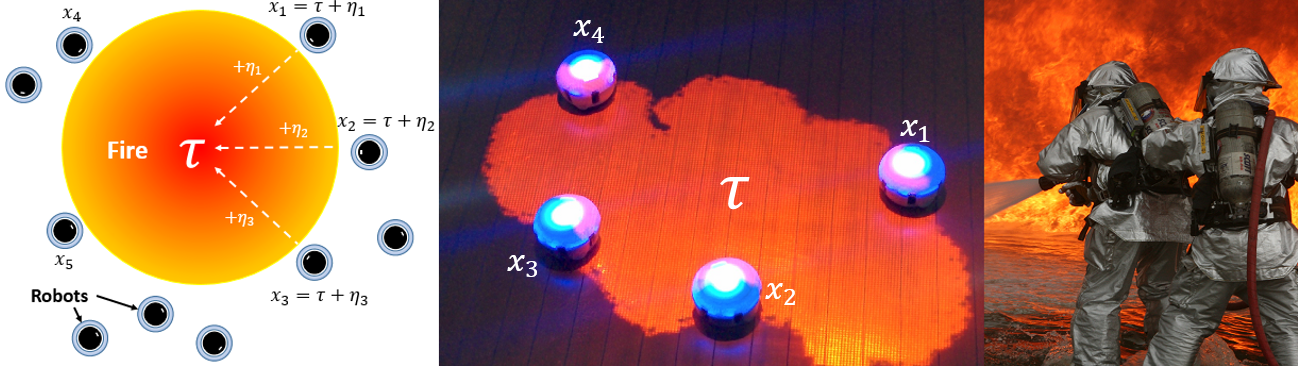
\includegraphics[width=\textwidth]{../figures/dropletfire.png}
\centering\caption{\textbf{Left:} A multi-robot firefighting scenario set up as a global game. Each player's imperfect estimate of the task is represented by $x_i$, a sum of the global magnitude parameter-$\tau$ and noisy sensor measurements-$\eta_i$. \textbf{Center:} The same scenario set up using actual robots and a projected fire, inspired from real forest fire containment (\textbf{Right}).}\label{fig:ggsetup}
\end{figure*}

\subsection{Formal Definition of a Concurrent Benefit Task}
We define a task $T$ to be a \textit{concurrent benefit task} if: 
\begin{enumerate}[a.]
	\item $u_i(1,g,\tau)-u_i(0,g,\tau)$ is an increasing and continuous function of $\tau$ for any $a_i\in A_i$ and $g$. We further assume that $|u_i(1,g,\tau)-u_i(0,g,\tau)|\leq \tau^p$ for some $p\geq 1$. 
	\item For extreme magnitude ranges, taking part in the activity is either appealing or repelling, i.e.\ there exists $\underline{\tau},\bar{\tau}\in (c,d)$ with $\underline{\tau}\leq \bar{\tau}$ such that for any $\tau\geq \bar{\tau}$, we have $u_i(1,g,\tau)>u_i(0,g,\tau)$ and for $\tau\leq \underline{\tau}$, the only equilibrium of the game is $(0,0,\ldots,0)$. 
\end{enumerate}

Note that in order to have such a task, we need the above conditions to hold for all the robots, i.e.\ for all $i\in\{1,\ldots,n\}$.
An example of a utility function that would satisfy such conditions is a function $u_i(a_i,g,\tau)=a_i(1-e^{-(g+1)}+\tau)$. Also, note that in a typical robotics scenario, the robots have a common utility function which is aligned with the system's objective. But in general, they may have different utility functions that need to satisfy the above conditions. 

The main challenge in devising strategies in performing a concurrent benefit task is that the knowledge of the magnitude parameter is not easily accessible to the robots. For example, consider the firefighting scenario described above. The magnitude of the task is not easily estimated by each robot and they only have noisy, imperfect information through their on-board sensors and their local measurements.  We model this imperfect knowledge by assuming that robot $i$ observes $x_i=\tau+\eta_i$ where $\eta_i$ is a Gaussian $\mathcal{N}(0,\sigma_i^2)$ random variable, as seen in Fig.~\ref{fig:ggsetup}. Throughout our discussion, we assume that the task magnitude $\tau$ is a Gaussian random variable\footnote{This analysis is extendable to a larger class of random variables but for the simplicity of the discussion, we consider Gaussian random variables here.} and it is independent of $\eta_1,\ldots,\eta_n$. Now, the main question is that given a robot's private measurement $x_i$, what is a \textit{sensible strategy} to follow. 

To define what a \textit{sensible strategy} is, let us first define what we mean by a \textit{strategy}. We refer to a function that maps measurements (observations) to actions $A_i$ as a strategy. Mathematically, a strategy $s_i$ for the $i$th robot is a (measurable) function $s_i:\R\to A_i$. Indeed a strategy $s_i$ prescribes what action the $i$th robot should take given its own measurement $x_i$. Given this, consider a set of robots with strategies $s_1,\ldots,s_n$. Let us denote the strategies of the $n-1$ robots other than the $i$th robot by the vector $s^{-i}=(s_1,\ldots,s_{i-1},s_{i+1},\ldots,s_n)$.  We say that a strategy $s_i$ is a threshold strategy if $s_i(x)=\text{step}(x-t_i)$ where $\text{step}(x)$ is the step function which is $1$ for $c\geq 0$ and $0$ for $c<0$.


For the $i$th robot, we define the best-response $BR(s^{-i})$ (to the strategies of the other robots) to be a strategy $\tilde{s}$ that for any $x\in \R$: 
\begin{align}\label{eqn:BR}
BR(s^{-i})(x)&=\tilde{s}(x)=\argmax_{a_i\in A_i} E(u_i(a_i,g,\tau)\mid x_i=x)\cr 
&=\argmax_{a_i\in A_i} E(u_i(a_i,\sum_{j\not=i}s_j(x_j),\tau)\mid x_i=x),
\end{align}
where $E(\cdot \mid x_i)$ is the conditional probability of $u_i$ given the $i$th agent's observation. Note that given $x_i$ and the strategies of the other robots $s^{-i}=(s_1,s_2,\ldots,s_{i-1},s_{i+1},\ldots,s_n)$, $\tau$, and $s_j(x_j)$ will be a random variable. In other words, given the $i$th robot's observation $x_i$, the observation of the other robots and hence, their actions would be random from the $i$th robot perspective.


Now, we are ready to define what we mean by a \textit{sensible strategy}. We say that a strategy profile $s=(s_1,\ldots,s_n)$ is a \textit{Bayesian Nash Equilibrium} (BNE) \cite{fudenberg1998theory} if $s_i=BR(s^{-i})$ for all $i\in \{1,\ldots,n\}$. In other words, with the current strategies of the $n$ robots, no robot has the incentive to deviate from its current strategy.

\subsection{Main Theorem and Proof}\label{sec:thmproof}
Here, we show that any task with concurrent benefits, admits a threshold strategy BNE. In other words, it is sufficient for the robots to follow a simple rule/algorithm: 
\begin{enumerate}[(i)]
\item Compare the measurements to a threshold value $\tau_i$,
\item If the measurement is above $\tau_i$ take part in the collaborative task, otherwise hold off. 
\end{enumerate}

In general, the existence of a BNE for a game is a questionable fact. Especially, once we impose additional constraints on the structure of strategies. However, in this case, we can show that there exists a sensible threshold policy for the class of tasks with concurrent benefits. To prove this, we show some intermediate results. 
\begin{lemma}\label{lemma:thresholdBR}
Let $s=(s_1,\ldots,s_n)$ is a strategy profile consisting of threshold strategies for a task with concurrent benefit. Let $\tilde{s}_i=BR(s^{-i})$. Then $\tilde{s}_i$ is a threshold policy. 
\end{lemma}
\begin{proof}
We first show that if for some observation $x_i=x$, we have $BR(s^{-i})(x)=\tilde{s}_i(x)=1$, then $\tilde{s}_i(y)=1$ for $y\geq x$. To show this,  we note that $P(x_j\geq \tau_j\mid x_i=x)$ is an increasing function of $x$ as $x_j-x_i$ is a normally distributed random variable. Therefore, using the monotone property of concurrent tasks and the fact that $x_i=\tau+\eta_i$, we conclude that 
\begin{align}
&E(u_i(1,\sum_{j\not=i}s_j(x_j),\tau)\mid x_i=y)\cr 
&\qquad-E(u_i(0,\sum_{j\not=i}s_j(x_j),\tau)\mid x_i=y)\cr 
&>E(u_i(1,\sum_{j\not=i}s_j(x_j),\tau)\mid x_i=x)\cr
&\qquad-E(u_i(0,\sum_{j\not=i}s_j(x_j),\tau)\mid x_i=x)\geq 0.
\end{align}
Therefore $\tilde{s}_i(y)=1$. Similarly, if for some value of $x$, we have $\tilde{s}_i(x)=0$, then it follows that $\tilde{s}_i(y)=0$ for $y\leq x$. Therefore, $\tilde{s}_i$ would be a threshold policy.  
\end{proof}

Based on the above lemma, we can view the best-response of threshold strategies as a mapping from $\R^n$ to $\R^n$ that maps $n$ thresholds of the original strategies to $n$ thresholds of the best-response strategies. With the abuse of notation, let's denote this mapping also by $L:\R^n\to\R^n$. The next step is to show that this mapping is a continuous mapping. 
\begin{lemma}\label{lemma:continuous}
The mapping $L$ described above is a continuous mapping. 
\end{lemma}
\begin{proof}
Let $x^{(-i)}=(x_1,\ldots,x_{i-1},x_{i+1},\ldots,x_n)$ be the vector of observations of $n-1$ robots except the $i$th robot. Note that the vector $(x^{-i},\tau)$ given $x_i=x$ is a normally distributed random vector which we denote its distribution by $f_{x}(x^{-i},\tau)$. Now, let $\{\alpha(k)\}$ be a sequence in $\R^n$ that is converging to $\alpha\in\R^n$. Let $\{\beta(k)\}$ be the sequence of thresholds corresponding to best-response strategy of a strategy with threshold vector $\alpha(k)$. Let $s$ be the threshold strategy corresponding to the threshold vector $\alpha$ and let $\alpha^*$ be the threshold policy corresponding to the $BR(\alpha)$. By the definition of the best-response strategy, $\beta_i(k)$ is a point where 
\begin{align}
&\int_{\R^{n}}f_{\beta(k)}(z,t)(u_i(1,\sum_{j\not=i}u^{\alpha_j(k)}(x_j),\tau)\cr 
&\qquad-u_i(1,\sum_{j\not=i}u^{\alpha_j(k)}(x_j),\tau))d(z\times t)=0.
\end{align}
Using the fact that $f$ has a Gaussian distribution and is continuous on all its arguments and the fact that $|u_i(\cdot,\cdot,\tau)|\leq \tau^p$, by taking the limit $k\to\infty$ and the dominated convergence theorem:
\begin{align}
&\int_{\R^{n}}f_{\beta}(z,t)(u_i(1,\sum_{j\not=i}u^{\alpha_j}(x_j),\tau)\cr 
&\qquad-u_i(1,\sum_{j\not=i}u^{\alpha(k)}(x_j),\tau))d(z\times t)=0,
\end{align}
where $u^{r}$ is a threshold strategy with threshold $r$. Therefore, the $\lim_{k\to\infty}L(\alpha(k))=L(\alpha)$ for a sequence $\alpha(k)$ that is converging to $\alpha$.
\end{proof}
Finally, we are ready to prove our main result. 

\begin{theorem}\label{thrm:mainthrm}
For a concurrent task $T$, suppose that the magnitude parameter $\tau$ is a Gaussian random variable. Also, suppose that $x_i=\tau+\eta_i$ where $\eta_1,\ldots,\eta_n$ are independent Gaussian random variables. Then, there exists a strategy profile $s=(s_1,\ldots,s_n)$ of threshold policies that is a Bayesian Nash Equilibrium.
\end{theorem}
\begin{proof}
By Lemma~\ref{lemma:thresholdBR}, the best response of a threshold policy is a threshold policy and hence, it induced the mapping $L$ from the space of thresholds ($\R^n$)to itself. Also, by Lemma~\ref{lemma:continuous}, this mapping is a continuous mapping. Now, if $t_i$ is sufficiently large threshold, then the second property of the concurrent benefit tasks implies that the $\tilde{t}_i\leq t_i$ because large enough measurement $x_i$ implies that agent $i$ itself should take part in the task. Similarly, for sufficiently low threshold $t_i$, we will have $\tilde{t}_i\geq t_i$. Therefore, the mapping $L$ maps a box $[a,b]^n$ to itself, where $a$ is a sufficiently small scalar and $b>a$ is a sufficiently large scalar. Since, a box $[a,b]^n$ is a convex set, by the Brouwer's fix point theorem \cite{border1990fixed}, we have that there exists a vector of threshold values $\alpha^*$ such that $L(\alpha^*)=L(\alpha^*)$ and hence, there exists a Bayesian Nash Equilibrium for a concurrent task $T$.
\end{proof}



\section{Why Sigmoid functions?}\label{sec:sigfun}
Sigmoid functions and decision making based on sigmoidal functions has been observed in many different settings in nature. [ANSHUL: please add some references and make the story more appealing here.] But the above discussion, seemingly, provides a different explanations to such observations. Here, we argue that not only Theorem~\ref{thrm:mainthrm} does not contradict such observations but also, provides a serious argument for prevalence of such phenomena. 

To explain this suppose that all the agents share the same utility function $u$ and also, assume that the observation noise of the $n$ agents ($\eta_1,\ldots,\eta_n$) are i.i.d.\ $\mathcal{N}(0,\sigma^2)$ Gaussian random variable. Many examples of multiagent systems in nature as well as swarm robotics satisfy such condition. Then, it is not hard to see that there exists a BNE with threshold strategies that have the same threshold value $\tau^*$ (see e.g.\ \cite{Morris2000}). Now, consider a realization of $\tau=\hat{\tau}$ and suppose that we have a large number of agents $n$ observing a noisy variation of $\hat{\tau}$. Take for example the case of an ant colony, and let $\hat{\tau}$ be a specific amount of pheromone. Then, since the observations of the $n$ agents are independent given the value of $\tau$, they will be distributed according to $\mathcal{N}(\hat{\tau},\sigma^2)$ (given the value of $\tau$). Now consider the relative number of agents taking part in the activity given the magnitude parameter $\hat{\tau}$.
\begin{equation}
	p_n(\hat{\tau})=\frac{\#\text{agents with }x_i\geq \tau^*}{n}
\end{equation}

Then, we have the following theorem.
\begin{theorem}\label{thrm:relativefrequency}
For the relative number of agents $p_n(\hat{\tau})$, we have
\begin{align}
\lim_{n\to\infty}p_n(\hat{\tau})=1-\Phi(\frac{\hat{\tau}-\tau^*}{\sigma^2})
\end{align}
where $\Phi$ is the cumulative distribution function (cdf) of a standard Gaussian. 
\end{theorem}
\begin{proof}
Note that $p_n(\hat{\tau})=\frac{1_{x_i\geq \tau^*}}{n}$ where $1_{\alpha\geq \beta}$ is the indicator function for $\alpha\geq \beta$. But note that for a given $\hat{\tau}$, $x_i$s are i.i.d.\ $\mathcal{N}(\hat{\tau},\sigma^2)$ random variables. Therefore, by the Gilvenko-Cantelli theorem \cite{durrett2010}, it follows that:
\begin{equation}
\lim_{n\to\infty}p_n(\hat{\tau})=1-F(\frac{\hat{\tau}-\tau^*}{\sigma^2})
\end{equation}

\end{proof}
Therefore, for large $n$, the relative frequency of agents taking part into the activity has a shape that follows the shape of the cdf of a standard Gaussian random variable and a frequentist interpretation of ant colony activity in such a setting is that the probability of an ant taking part in the activity roughly follows the curve of this function. 

The final step to explain the prevalence of sigmoidal functions in multiagent settings is to note that:
\begin{align}
|\Phi(x)-\frac{1}{1+e^{-1.702x}}|\leq 0.01,
\end{align}
for all $x\in\R$ (see \cite{camilli1994} and the references therein). Note that $\frac{1}{1+e^{-dx}}$ is the standard, logistic sigmoid function. 



\section{Discussion}\label{sec:disc}
1. The proof uses a step-function as the threshold function. In biological insect colony models and some swarm task-allocation models (including our own) we use continuous threshold functions (like sigmoid). I would like to address this in the Discussion section and bridge the gap between step-functions and sigmoid functions by saying that a step-function is just an extreme case of a continuous sigmoid function as it's slope goes to infinity. Do you see this causing any logical issue with your proof? I can see that this makes the analysis of the pure-thershold strategy $s_i$ more difficult. Can we somehow fold in continuous threshold functions into the global games setting, as part of the proof?

There is a story there, we can tell that we are considering the ideal case where each agent knows how many other agents are in the field as well as information sharing. Then we can say, this is the prescription for the ideal case, for the non-ideal scenario of not knowing how many agents are in the field and also information sharing, sigmoid function is an engineering solution. Perhaps you wanna discuss it as future direction. 

2. I will talk about the restriction of no information sharing between agents in the Discussion section as well. There has been some work done in analysing global games with sharing of information between agents, right? I'd like to reference that work if possible as an avenue for future research.

Regarding information sharing, there is one work of mine and Jeff which is on this topic \cite{Touri2014}.

3. Coming back to the discussion of "system equilibrium" vs. "system optimum". Can we say anything about an optimal task-allocation strategy in this paper? I'd like to draw a clear separation between these two concepts in the discussion section as well. 

This is definitely very interesting but it is hard to say anything mathematically. The system optimum is something that one should define. One definition would be the optimal task allocation once a central agent knows all the information (sensor measurements, number of agents,…) in the system. It’s performance would be definitely much better than none central allocation and this setting of global games where the information is shared globally. 

\section{Conclusion}\label{sec:conc}
We have formulated robotic task allocation in the context of game theory, and showed how a common class of tasks can be reduced to a global game. Using this framework, we have shown that a threshold-based policy, which is commonly observed in social insects and successfully used in swarm robotics, can indeed be considered an optimal policy if the robots cannot communicate. 



%%%%%%%%%%%%%%%%%%%%%%%%%%%%%%%%%%%%%%%%%%%%%%%%%%%%%%%%%%%%%%%%%%%%%%%%%%%%%%%%
%%%%%%%%%   The Bibliography, if any   %%%%%%%%%
\bibliographystyle{IEEEtran}		% or "siam", or "alpha", etc.
%\nocite{*}
\bibliography{../refworks}
\end{document}
